\lampiransection{Poster Rekrutmen Informan Wawancara Pelanggan}
\label{app:poster-rekrutmen-informan-pelanggan}

Lampiran ini memuat poster rekrutmen informan pelanggan yang digunakan untuk mencari responden wawancara singkat terkait pengalaman membeli Nasi Gerilya. Poster ini ditujukan kepada calon informan yang memenuhi kriteria penelitian, yaitu pelanggan yang pernah atau bersedia melakukan pembelian Nasi Gerilya melalui GrabFood dan kemudian memberikan keterangan berdasarkan pengalaman aktual.

\begin{table}[!htbp]
    \centering
    \caption{Identitas Poster Rekrutmen Informan Pelanggan}
    \label{tab:identitas-poster-rekrutmen-informan-pelanggan}
    \begin{tabularx}{\textwidth}{|Z{3.4cm}|Y|}
        \toprule
        \textbf{Aspek} & \textbf{Keterangan} \\ \hline
        \midrule
        Media & Poster ajakan wawancara pelanggan \\ \hline
        Sasaran & Pelanggan atau calon pelanggan Nasi Gerilya yang memenuhi kriteria informan penelitian \\ \hline
        Tujuan & Mengundang informan untuk mengikuti wawancara singkat mengenai pengalaman dan persepsi terhadap Nasi Gerilya \\ \hline
        Insentif & Saldo GoPay Rp50.000 bagi informan yang memenuhi kriteria dan mengikuti wawancara \\ \hline
        Durasi & Sekitar 10 menit \\ \hline
        Kontak & 0812 6394 2491 \\ \hline
        Catatan etika & Informan tetap diberi kebebasan menjawab secara jujur, termasuk menyampaikan pengalaman positif maupun negatif. \\ \hline
        \bottomrule
    \end{tabularx}
    \tablesource{Diolah peneliti sebagai media rekrutmen informan pelanggan (2026).}
\end{table}

\clearpage
\begin{center}
\begin{minipage}{\textwidth}
\centering
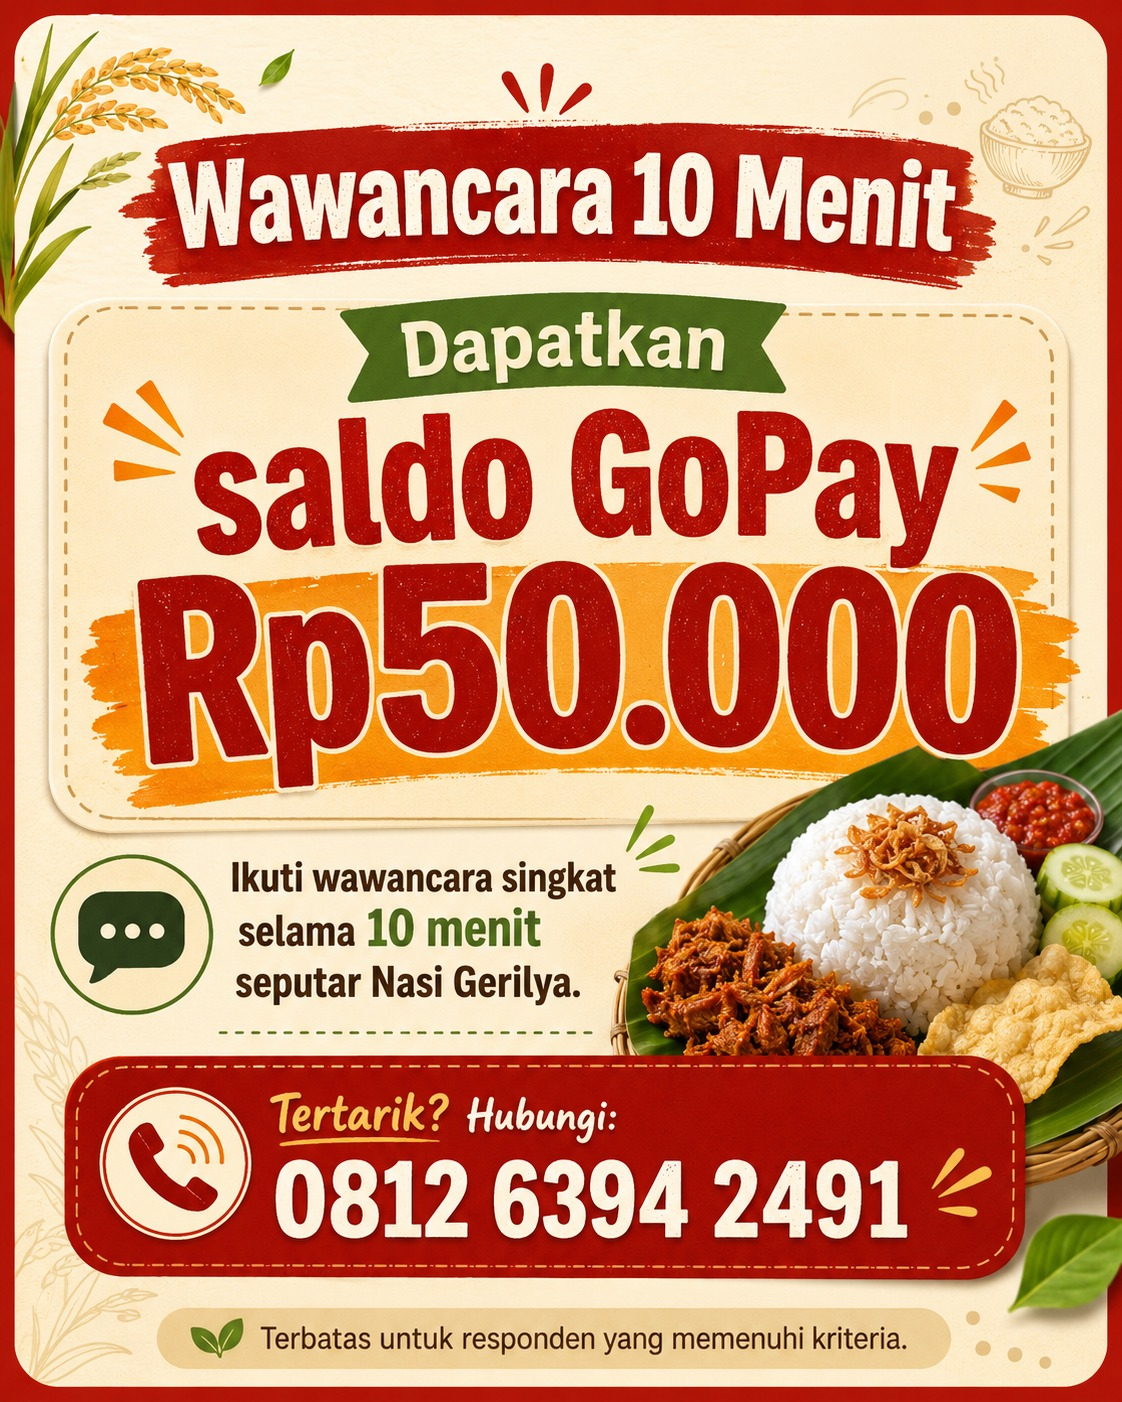
\includegraphics[width=0.82\textwidth,height=0.74\textheight,keepaspectratio]{resource/05-fieldwork/03-rekrutmen-informan/poster-rekrutmen-informan-pelanggan.jpeg}\par
\figuresource[0.82\textwidth]{Dokumentasi poster rekrutmen informan pelanggan Nasi Gerilya; diolah peneliti (2026).}
\captionof{figure}{Poster rekrutmen informan wawancara pelanggan Nasi Gerilya}
\label{fig:poster-rekrutmen-informan-pelanggan}
\end{minipage}
\end{center}
